
    \begin{abstract_online}{A Thermodynamic Perspective of Order-Disorder Transition of $\mathbf{Ni_3Fe}$ }{%
        \underline{A. Mangla}, G. Deo, P. A. Apte}{%
        }{%
        Department of Chemical Engineering, IIT Kanpur, India}
    The order—disorder (OD) transition temperature of $Ni_3Fe$ $(\approx 779 \ K)$ is well known from several experimental investigations primarily based on Mossbauer spectroscopy (MS) and electrical resistivity measurements [1,2]. Across $T_O$, $Ni_3Fe$ undergoes a transition from a disordered solid solution with a FCC structure to an ordered intermetallic compound with a $L_{12}$ structure (in which Fe atoms are at the corners and Ni atoms are at the face centers of the FCC lattice).  Here we investigate the mechanism of the transition with molecular simulations using two potentials based on embedded atom method (EAM).  One of the EAM potentials includes angular dependent terms which are considered crucial in case of Fe based alloys.  Although the OD transition temperatures are higher than the actual value, the alloys simulated using both the potentials show qualitatively similar mechanism.   As the alloy is cooled from the disordered state to the transition temperature $T_O$, there is a large increase in Fe and Ni atoms with $L_{12}$ local order that does not exceed beyond third coordination shell. There is a significant change in the bulk density and the long range order parameter (LROP), which increases from 0 in the disordered state to about 0.85 at $T_O$.  However the size of the $L_{12}$ ordered domains and hence the $L_{12}$ global order does not increase significantly.  Across $T_O$, $L_{12}$ ordered domains gain critical strength to overcome thermal fluctuations.   This is supported by the fact that the number of bulk sites of the $L_{12}$ ordered domains exhibit an inflection at $T_O$ and increase relatively rapidly as the temperature is reduced below $T_O$.  We find that the mechanism is similar to that of crystallization across the limit of stability of super cooled tetrahedral liquids such as silicon and water [3]. Such a mechanism, as found by earlier simulation studies, involves freezing of the tetrahedral network (against thermal fluctuations) followed by rapid growth of the network as the temperature is reduced across the stability limit.  Our results indicate that OD transition temperature $T_O$ in the actual $Ni_3Fe$ alloy, from a thermodynamic perspective, is possibly lower than the temperature across which sharp changes (due to $L_{12}$ local order) are observed in the LROP as well as in the bulk density.  \begin{center}  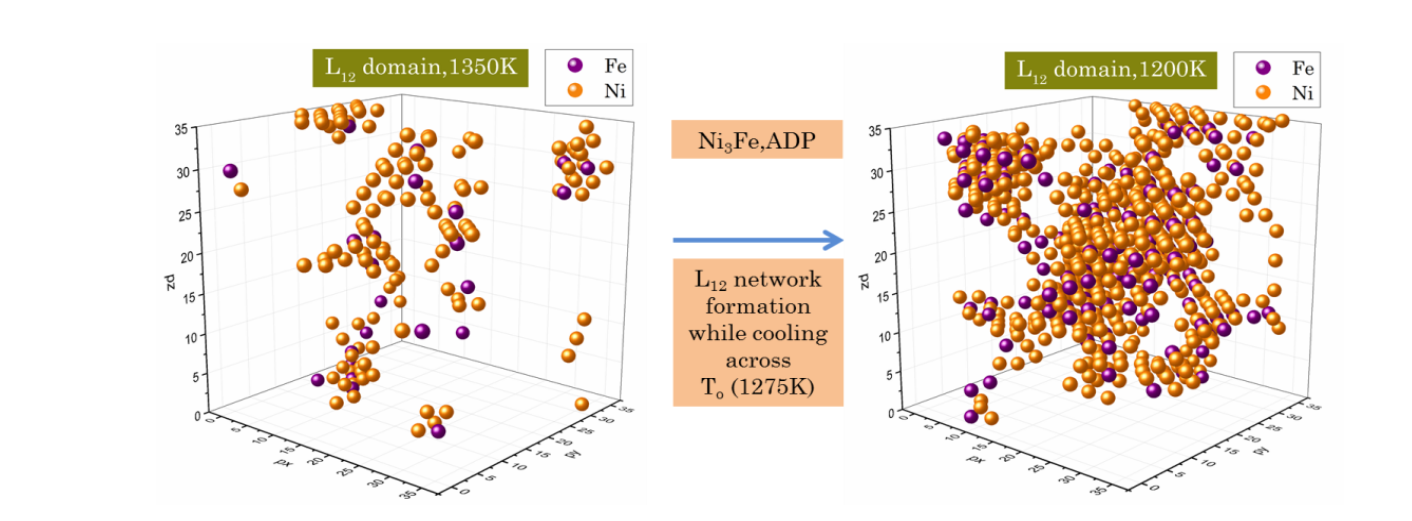
\includegraphics[width=\linewidth]{abstracts/txt/figures/anil.png}  \caption{\textbf{Figure 1:} On cooling, $L_{12}$ domain (global $Ni_3Fe$ order) increases steeply across transition temperature $(T_O)$. Above figure is generated using ADP force field for $Ni_3Fe$ system.}  \end{center} 
    
        \textbf{References} \newline{}[1] Drijver, J. W.,et.al., Phys. Rev. Lett. 34, 1026–1029 (1975).\newline{}[2]	Wakelin, R. J., et.al. Proc. Phys. Soc. Sect. B 66, 221–240 (1953).\newline{}[3]	Pingua, N., et.al. J. Chem. Phys. 149, 074506 (2018).
    \end{abstract_online}
    